\subsection{Simplified and original Ikeda method}
\label{se:si_ikeda_model}
Comparing results from the SI-method with corresponding results with the original Ikeda's method can be a way to see if the observed deviations are from extrapolation or originates from the original method. In the Ikeda's method more detailed information about the ship hull geometry is needed, so that $B_W$ can be calculated with a strip method and $B_E$ can be calculated using sectional lewis coefficients. It was possible to collect the required hull inputs for 15 ships in the database. These ships were used in 50 of the reference roll decay tests, where all but one of the tests exceed the limits. Ikeda method has a much better agreement for these exceeding model tests accoding to figure \ref{fig:si_ikeda_model} and the calculated $R^2$ in table \ref{tab:si_ikeda_validation}.


When comparing the damping components from SI and Ikeda (Fig.\ref{fig:component_residual}) $B_W$ seem to be the main cause of the SI error. When also looking how the error changes with input parameters (Fig.\ref{fig:parameter_residual}) it seems that the error is large when the beam to draught ratio (and consequently also $\hat{\omega}$) is large. This is shown in more detailed in figure \ref{fig:beam_T_residual} where the error is increasing when the beam to draught ratio is above 4.5. This makes a lot of sense when looking back on the input parameter variation in figure \ref{fig:SI_sensitivity} where enormous values of $B_W$ were observed above this value, which also happens to be the limit value according to Eq.\ref{eq:SI_limits}.

\begin{figure}[H]

    \centering
    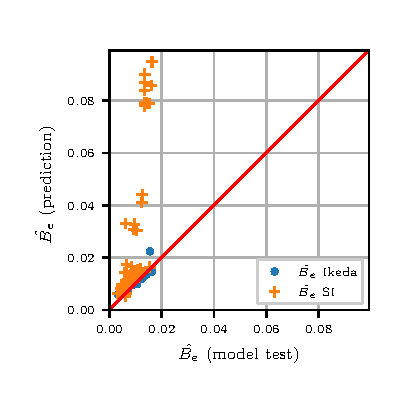
\includegraphics[width=0.5\textwidth]{figures/si_ikeda_model.eps}
    \caption{Comparison SI, Ikeda and model tests}
    \label{fig:si_ikeda_model}

\end{figure}


\begin{table}[H]
    \centering
    \caption{Validation of SI and Ikeda}
   \begin{tabular}{lrr}
\toprule
{} &   $R^2$ &  Number of points \\
\midrule
Ikeda        &    0.84 &               500 \\
SI no limits & -127.95 &               500 \\
\bottomrule
\end{tabular}

    \label{tab:si_ikeda_validation}
\end{table}
    

